\documentclass{acm_proc_article-sp}
\usepackage[table]{xcolor}
\usepackage{graphicx}
\usepackage{hyperref}
\hypersetup{
    colorlinks = false,
    pdfborder = {0 0 0},
}

\makeatletter
\newif\if@restonecol
\makeatother
\let\algorithm\relax
\let\endalgorithm\relax
\usepackage{algorithm2e}

\begin{document}

\title{Web Content Extraction Through Machine Learning
\titlenote{Source code for this project is avaiable on GitHub under the MIT License at \url{https://github.com/ziyan/spider}}}

\numberofauthors{2}
\author{
\alignauthor
Ziyan Zhou\\
\email{ziyanjoe@stanford.edu}
\alignauthor
Muntasir Mashuq\\
\email{muntasir@stanford.edu}
}

\maketitle

\begin{abstract}
Web content extraction is a key technology for enabling an array of applications aimed at understanding the web. While automated web extraction has been studied extensively, they often focus on extracting structured data that appear multiple times on a single webpage, like product catalogs. This project aims to extract less structured web content, like news articles, that appear only once in noisy webpages. Our approach classifies text blocks using a mixture of visual and language independent features. In addition, a pipeline is devised to automatically label datapoints through clustering where each cluster is scored based on its relevance to the webpage description extracted from the meta tags, and datapoints in the best cluster are selected as positive training examples.
\end{abstract}

\keywords{Content Extraction; SVM; DBSCAN; Web Scraping}

\section{Introduction}

Content extraction algorithms have been well studied and there are many interesting and useful applications\cite{diffbot}\cite{readability}. A survey by Laender et al.\cite{laender:brief} systematically covers a wide range of techniques used for this purpose. The techniques range from wrapper development to NLP-based and modeling-based approach. Miao et al.\cite{gengxin:extracting} proposed a fully automatic tag path clustering approach to extract structures on a single webpage. Sun et al.\cite{sun2011dom} applied a language independent approach by looking at text density at each area of the document.

We wanted to take a different approach to this problem. Our goal is to extract content of a webpage in a language independent way. We wanted to understand how we (humans) can identify the main content of a webpage even if we do not recognize the language of the website. The relevant information for us for those webpages are: visual features like font size, color and style; line spacing and block size; layout of the webpage; text density in different parts of webpage; density of links etc. In our algorithm we have used these visual features to train a SVM classifier to find out the content of a webpage.

Another aspect of our approach is that we wanted to run the complete pipeline automatically, from data collection \textemdash labeling\textemdash learning\textemdash testing. Specially we tried to avoid manual labeling of the dataset. So we devised a method using clustering to label the dataset.

Our overall algorithm looks like follows: label the collected dataset using clustering, train SVM with the labeled dataset, use SVM model to extract content from new webpages.

\section{Terminology}
Lets define a few terminology that would help us to understand the rest of the paper.
\subsection{Webpage}
A webpage is a document that is rendered by a browser corresponding to an URL.
\subsection{Block}
\label{subsec:block}
A block is part of a webpage that contains text and have both height and width. For example, a paragraph in the content of a webpage, a navigational link in menu, title of an article\textemdash each of these are separate blocks. The blocks are highlighed in \emph{Figure \ref{figure:blocks}}.

\emph{Each block is an input datapoint to our clustering and SVM algorithm.}

\subsection{Content}
Content is the main text of a webpage that we aim to extract. In content extraction literature, it is often referred as \emph{gold text}.

\section{Data Collection}

\begin{table}
\rowcolors{2}{gray!25}{white}
\centering
\caption{\label{table:dataset}Collected Dataset}
\begin{tabular}{|l|l|c|} \hline
Website&Language&\# of Webpages\\ \hline\hline
NPR&English&25\\ \hline
Prothom Alo&Begali&24\\ \hline
QQ&Simplified Chinese&25\\ \hline
Sina&Simplified Chinese&25\\ \hline
TechCrunch&English&16\\ \hline
The Verge&English&16\\ \hline
USA Today&English&20\\ \hline
Chaos&Mixed, includes RTL&189\\ \hline
\end{tabular}
\end{table}

The dataset is extracted from several popular English, Simplified Chinese, and Bengali news article websites on the Internet.\footnote{The collected dataset is available at \url{https://github.com/ziyan/spider/tree/master/data}} The Chaos dataset URLs are collected from Sun et al.\cite{sun2011dom} This dataset contains URLs from diverse websites across the Internet, such as, personal blogs, articles, news etc. See \emph{Table \ref{table:dataset}} for some information about our dataset.

For all the dataset, we collected the URLs and then extracted the webpage ourselves, as various existing dataset often cleans up the HTML and removes CSS properties that we need. Each webpage is downloaded and rendered in a virtual webkit browser\cite{phantomjs}, restoring its original layout intended for human audience. Javascript is then injected into the webpage to efficiently inspect DOM elements. Text enclosing blocks are identified. For each DOM element containing text, the algorithm finds its closest parent element that are displayed as block. Inline links and other text decorators are not individually identified. Instead, their common parent element, which might be a paragraph or a div, is identified as a whole. See \emph{Figure \ref{figure:blocks}}.

For each chosen block, a set of features are then extracted, including the size and position of the block, the contained text, the font configurations, color, line height, tag path, etc. In fact, there are over 300 different CSS properties for each block. Our algorithm automatically extracts those with a \emph{non-default} value. Therefore, the number of features varies from block to block in the data collection phase.


\begin{figure}[htp]
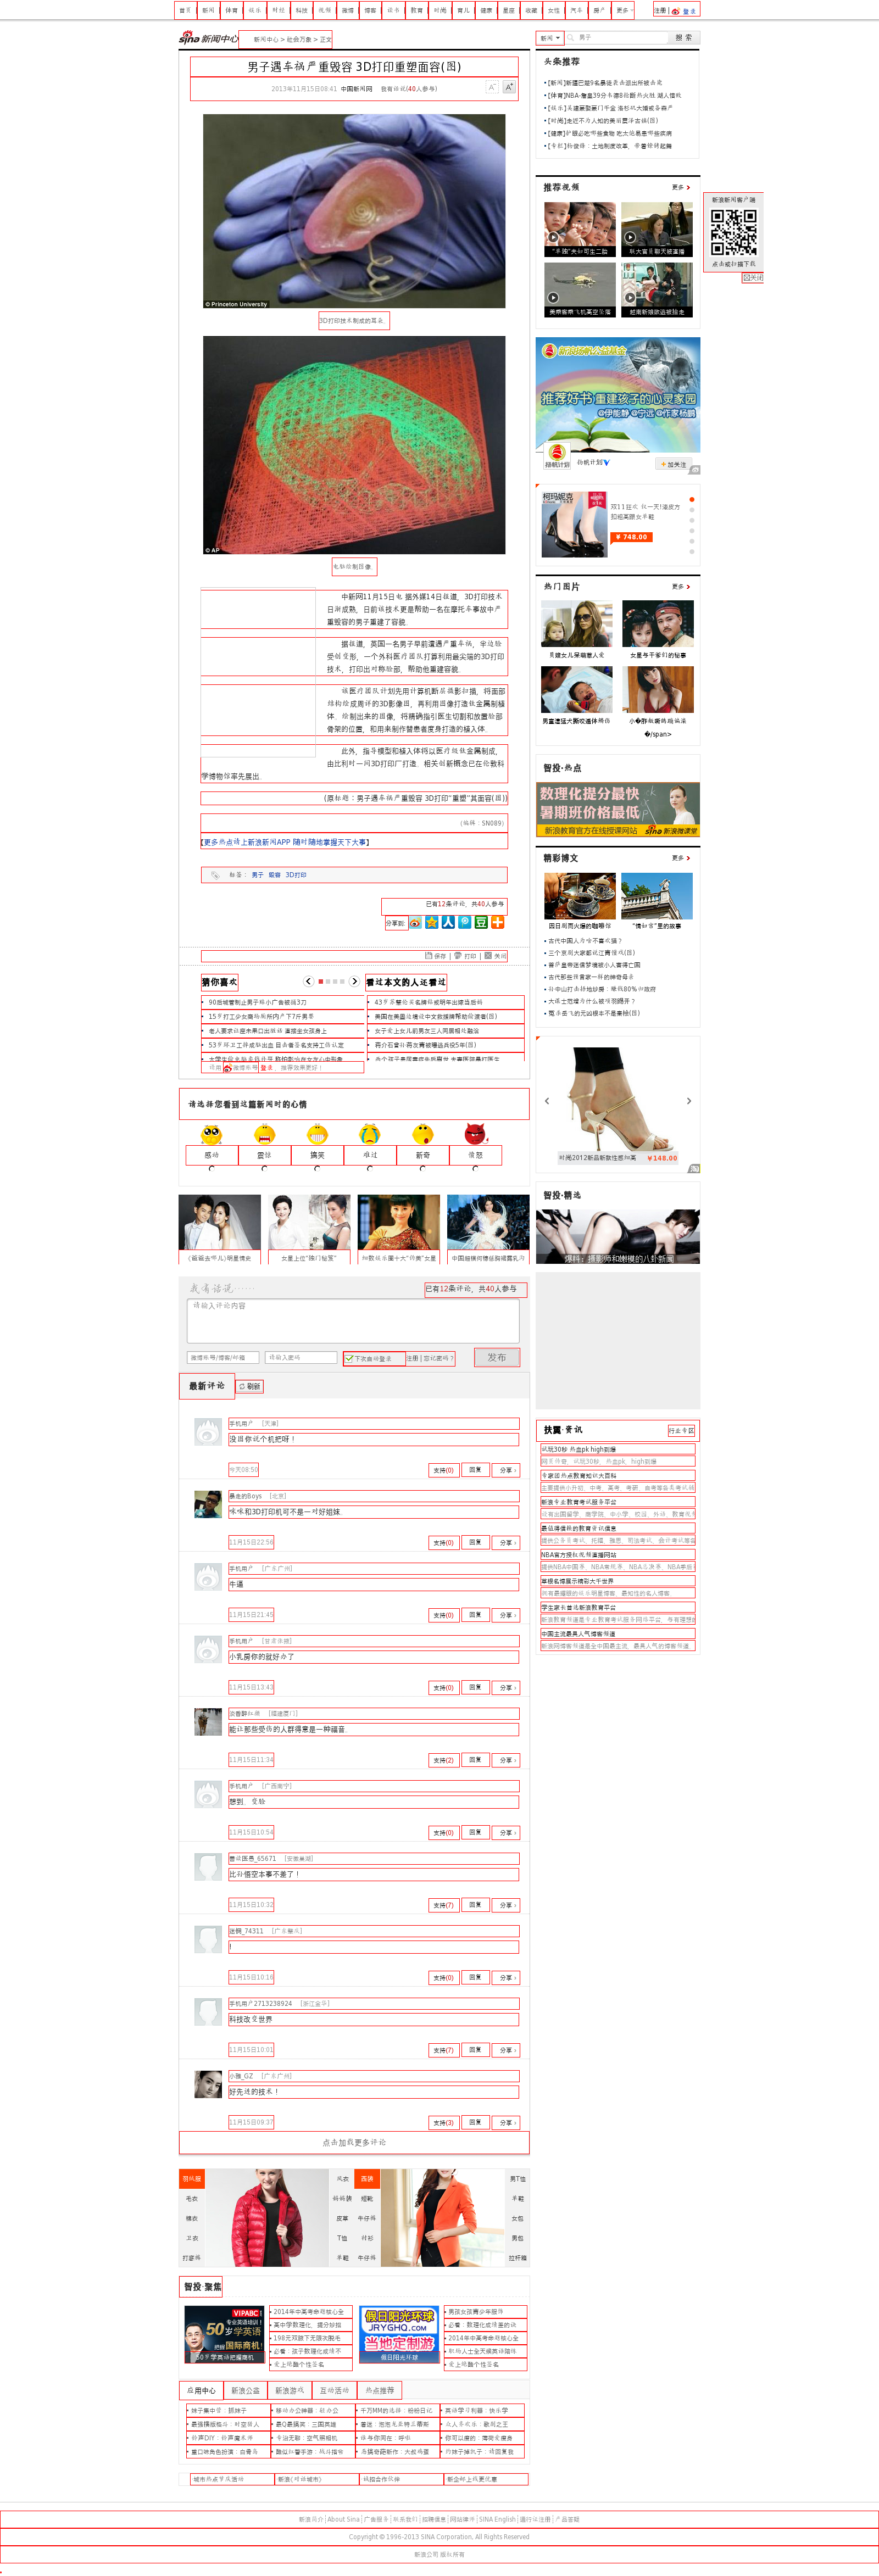
\includegraphics[scale=0.22]{blocks}
\caption{\label{figure:blocks}Webpage rendered by virtual webkit browser with text blocks identified by red boxes}
\end{figure}

\section{Automatic Labeling}


\subsection{Clustering Blocks}

The cluster shape of similar blocks on a webpage (i.e. navigational buttons) are not necessarily well-shaped (i.e. spherical). Also there can be random noises that appears on some of the webpages. Furthermore, it is  unclear that how many clusters will there be, since it depends heavily on the design and layout of the webpage. Therefore, we have chosen DBSCAN\cite{ester:dbscan}, density-based spatial clustering of applications with noise, as our clustering algorithm. This algorithm handles the problems of unknown number of clusters, unknown shape of clusters and noise quite nicely.

The clustering result shows that, the body text of the articles across multiple webpages, which usually consist of multiple blocks, are clustered together in a single cluster. The navigational links are also clustered together, as well as the links in the footers. Other common elements, like similar sidebar, advertisement, comments, etc., are also successfully clustered. Given all the visual features represented by the CSS properties, the algorithm is quite effective in discerning the different visual elements on the webpages.

\newpage
\begin{table}
\rowcolors{2}{gray!25}{white}
\centering
\caption{\label{table:approach1}Separate classifier for different website}
\begin{tabular}{|l|r|r|r|} \hline
Website&Precision&Recall&$F_1$\\ \hline\hline
NPR&100.00\%&100.00\%&100.00\%\\ \hline
Prothom Alo&100.00\%&100.00\%&100.00\%\\ \hline
QQ&100.00\%&100.00\%&100.00\%\\ \hline
Sina&100.00\%&100.00\%&100.00\%\\ \hline
TechCrunch&100.00\%&100.00\%&100.00\%\\ \hline
The Verge&100.00\%&100.00\%&100.00\%\\ \hline
USA Today&100.00\%&100.00\%&100.00\%\\ \hline
\end{tabular}
\end{table}


\subsection{Labeling Clustered Block}
Although all the blocks have been clustered quite precisely based on their visual properties, it is not trivial to find out which cluster contains the content text. The DBSCAN algorithm views clusters as areas of high density separated by areas of low density. Cluster number varies from webpage to webpage, and the cluster containing content can be any of those. For our dataset, the number of output clusters ranges from a few clusters to above 20.

Fortunately, most websites have some metadata stored in meta tags in order to accommodate web crawlers. So we can extract the \emph{description} of an article by parsing the meta tags in the webpage. The description usually contains a brief summary or just the first few words of the article content. With that, we are able to calculate the similarity between each cluster and the \emph{description} using the Longest Common Sub-sequence (LCS) algorithm. The longer the common sub-sequence (we call this number ``relevance score''), the more likely is the cluster to contain the content text. Note that we used LCS instead of Term Frequency or Inverse Document Frequency to ensure the language independence, as word segmentation varies from language to language.

At first we tried to automatically label the blocks by finding the best cluster local to each webpage on a website. After training the SVM on this labeling, we found that for some websites, the precision on the test set was not ideal. On closer examination, we found that on some rare pages, the best cluster according to that webpage's description is comment instead of the main text. To fix this issue, we implemented \emph{Algorithm \ref{algorithm:1}} which scores the blocks across the entire website (rather than working locally on a single webpage).

\begin{algorithm}
\caption{\label{algorithm:1}Labeling from global score in a website}
 %\SetLine
 score := {array of zeros with length equal to \# of clusters}\;
 \For{each cluster i of a website}{
  \For{each block j under that cluster}{
    score[i] := score[i] + relevance score of block j\;
  }
 }
 Pick the cluster(C) with the highest similarity score\;
 Label all the blocks of in the same cluster C as 1\;
 Label all other blocks as 0\;

\end{algorithm}

This algorithm performs very accurately and removes the occasional labeling hiccups on a single webpage.



\begin{table}
\rowcolors{2}{gray!25}{white}
\centering
\caption{\label{table:approach2}Testing on previously unseen websites}
\begin{tabular}{|l|r|r|r|} \hline
Dataset&Precision&Recall&$F_1$\\ \hline\hline
Chaos&71.75\%&20.65\%&31.28\%\\ \hline
\end{tabular}
\end{table}

\begin{table}
\rowcolors{2}{gray!25}{white}
\centering
\caption{\label{table:approach3}Using random mixture of webpages}
\begin{tabular}{|l|r|r|r|} \hline
Dataset&Precision&Recall&$F_1$\\ \hline\hline
Chaos&96.86\%&89.64\%&92.83\%\\ \hline
\end{tabular}
\end{table}

\newpage
\section{SVM and Cross Validation}

Using the collected and labeled text blocks, the web content extraction problem can be formulated as a classification problem, where the goal content consists of multiple text blocks that are classified as content while the other text blocks are classified as non-content.

We have constructed a support vector classifier with a linear kernel to perform text block classification. Due to the imbalance between the number of content blocks and the number of non-content blocks on a webpage, we applied class weights to give our positive (content) examples higher weights.

We have employed three different approaches to the classification problem. For each approach, we have performed 4-fold cross validation to evaluate its performance.

In our first approach, we have trained separate classifier for different website. For each given website, the collected webpages are shuffled then divided into four groups. One of the groups is chosen as evaluation group, while the other three are used as training examples. Intuitively, the support vector classifier in this case tries to learn the underlying structure and template used by the particular website. This approach worked very well. See \emph{Table \ref{table:approach1}}.

In our second approach, we have trained one classifier model using webpages from multiple websites in the chaos dataset and then tested the model on webpages from the rest of the dataset. The classifier in this case learns some structures from only a subset of websites then tries to generalize the model on previously unseen websites. This approach produced the worst results. See \emph{Table \ref{table:approach2}}. It make sense that specific visual characteristics of one website rarely appears the same in another website.

And lastly, we have trained one classifier model using random webpages chosen from the chaos dataset then tested the model on the rest of the dataset. In this approach, since the webpages used in training are picked randomly, our training examples included a wide variety of websites. Therefore, it is likely that the classifier have previously seen at least one example webpage per website for the websites in the evaluation set. This approach worked much better than the second approach. See \emph{Table \ref{table:approach3}}.

The results from the third approach has shown that our algorithm is able to learn and generalize more than one template at a time. Combined with results from the first approach, these results indicate that our algorithm will work well for any website including websites using multiple different templates as long as the classifier is trained on a representative mixture of example webpages.


\section{Feature Selection}

In order to develop deeper insights into our classification problem, we experimented with different feature sets.


\begin{table}
\rowcolors{2}{gray!25}{white}
\centering
\caption{\label{table:textlength}Using text lengths as features}
\begin{tabular}{|l|r|r|r|} \hline
Website&Precision&Recall&$F_1$\\ \hline\hline
NPR&78.99\%&91.34\%&84.70\%\\ \hline
Prothom Alo&42.14\%&75.01\%&53.31\%\\ \hline
QQ&31.95\%&75.43\%&44.70\%\\ \hline
Sina&62.92\%&60.63\%&61.69\%\\ \hline
TechCrunch&32.84\%&83.18\%&46.96\%\\ \hline
The Verge&53.56\%&86.86\%&66.08\%\\ \hline
USA Today&75.45\%&82.98\%&78.83\%\\ \hline
\end{tabular}
\end{table}

\begin{table}
\rowcolors{2}{gray!25}{white}
\centering
\caption{\label{table:tagpath}Using tag paths as features}
\begin{tabular}{|l|r|r|r|} \hline
Website&Precision&Recall&$F_1$\\ \hline\hline
NPR&99.74\%&100.00\%&99.87\%\\ \hline
Prothom Alo&100.00\%&100.00\%&100.00\%\\ \hline
QQ&58.68\%&100.00\%&73.88\%\\ \hline
Sina&94.61\%&100.00\%&97.22\%\\ \hline
TechCrunch&100.00\%&100.00\%&100.00\%\\ \hline
The Verge&92.34\%&100.00\%&96.00\%\\ \hline
USA Today&100.00\%&100.00\%&100.00\%\\ \hline
\end{tabular}
\end{table}

\begin{table}[t]
\rowcolors{2}{gray!25}{white}
\centering
\caption{\label{table:selectors}Using CSS selectors as features}
\begin{tabular}{|l|r|r|r|} \hline
Website&Precision&Recall&$F_1$\\ \hline\hline
NPR&100.00\%&100.00\%&100.00\%\\ \hline
Prothom Alo&100.00\%&97.79\%&98.87\%\\ \hline
QQ&61.74\%&100.00\%&73.94\%\\ \hline
Sina&97.56\%&100.00\%&98.76\%\\ \hline
TechCrunch&100.00\%&100.00\%&100.00\%\\ \hline
The Verge&100.00\%&96.21\%&97.95\%\\ \hline
USA Today&100.00\%&98.29\%&99.11\%\\ \hline
\end{tabular}
\end{table}

\begin{table}[t]
\rowcolors{2}{gray!25}{white}
\centering
\caption{\label{table:css}Using CSS visual properties as features}
\begin{tabular}{|l|r|r|r|} \hline
Website&Precision&Recall&$F_1$\\ \hline\hline
NPR&100.00\%&100.00\%&100.00\%\\ \hline
Prothom Alo&100.00\%&100.00\%&100.00\%\\ \hline
QQ&100.00\%&100.00\%&100.00\%\\ \hline
Sina&100.00\%&100.00\%&100.00\%\\ \hline
TechCrunch&94.27\%&100.00\%&97.03\%\\ \hline
The Verge&100.00\%&100.00\%&100.00\%\\ \hline
USA Today&100.00\%&100.00\%&100.00\%\\ \hline
\end{tabular}
\end{table}

\subsection{Text Length}

A common naive approach to web content extraction is to find the longest contiguous block of text in a webpage. The intuition is that paragraphs in an article are usually long. To establish some baseline, we've experimented with using only text length as feature. The text length of each text block is simply the number of non-whitespace characters in the block. We normalize this number by scaling it to have a zero mean and a variance of one.

The results show that this approach works for some websites but performs quite poorly for others. See \emph{Table \ref{table:textlength}}. Due to the variation of paragraph length in the real world, text length is not a very good determinator of article content.

\subsection{Tag Path}

The second approach is to use tag path of the block. Tag path is simply the path it takes to navigate the DOM tree from its root to the text block. It consists of element names for each node along the path. For example, a paragraph inside a $div$ container in the $body$ of the HTML webpage would have a tag path like \emph{``body > div > p''}. We treat each different tag path uniquely and vectorized this discrete feature.

The results show that this approach works quite well in general but fails for some particular website. We found that in the failure cases, the tag paths are indeed indistinguishable for content and some non-content text blocks. Therefore, this feature alone cannot sufficiently distinguish the two classes of blocks. See \emph{Table \ref{table:tagpath}}.

\subsection{CSS Selectors}

CSS selectors are essentially decorated tag paths. We have incorporated CSS class name in addition to the element name into the CSS selectors. These selectors have the potential to discriminate previously indistinguishable text blocks, thus allowing the classifier extract more concise template information for a given website.

The results shows that this approach produces improvement for most of the websites compared to the tag path approach, but also introduces some regressions for other. See \emph{Table \ref{table:selectors}}. Upon closer examination, we learned that some CSS selectors can be overly unique and tied only to a particular text block. Its idiosyncrasy presents a challenge for the classification model to generalize to other text blocks.

\subsection{CSS Properties}

The third approach is to use all visual related CSS properties (color, font-size, font-style, line-height etc.) as features. These features are also treated as discrete features and vectorized.

The results show that similar to tag path and CSS selectors, these features work quite well in general but not ideal in some rare cases. Especially for websites that do not visually distinguish content with other parts of the webpage, these visual features alone are not sufficient. See \emph{Table \ref{table:css}}.


\section{Conclusion}

We have developed a language independent pipeline to extract web content. Our pipeline collects data, labels examples, trains support vector classifier, and evaluates learned model in an automated manner. Our learning algorithm can achieve perfect labeling when trained on a single website, even for websites with multiple different templates. By analyzing features, we have found that some of our features\textemdash tag path, CSS selectors\textemdash contributed to the near perfect classification results in many websites, but they also fail in some cases. CSS visual properties work particularly well across most websites. This reinforces the intuitive reasoning about how a person identifies the content in a website. Tag path and CSS selectors are technical details of presenting HTML documents, which often matches with human intuitive reasoning but may break in times. See \emph{Table \ref{table:approach1}}.

\section{Future Work}
Sun et al.\cite{sun2011dom} showed the interesting idea of density sum in his paper. Density sum performs very well in Chaos dataset (F1 score: 96.15\%) It would be interesting to see how combination of density sum and CSS features perform. But we need to refactor our code extensively to incorporate density sum, so we were not able do it in the current time frame.







\bibliographystyle{abbrv}
\bibliography{final}


\end{document}

